\definecolor{Purple}{RGB}{120,28,129}
\definecolor{Blue}{RGB}{63,96,174}
\definecolor{Duck}{RGB}{83,158,182}
\definecolor{Green}{RGB}{109,179,136}
\definecolor{Yellow}{RGB}{202,184,67}
\definecolor{Orange}{RGB}{231,133,50}
\definecolor{Red}{RGB}{217,33,32}
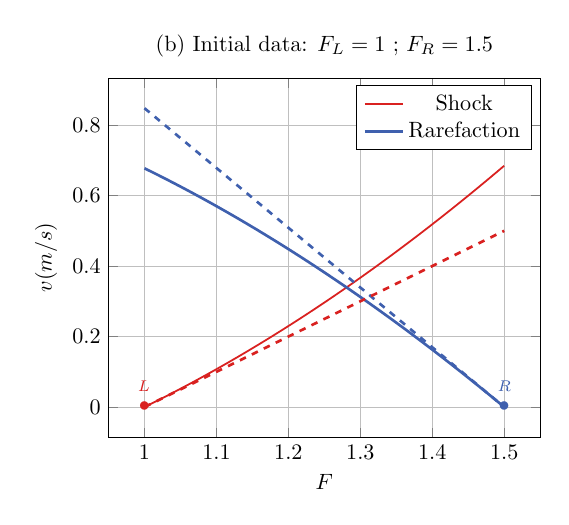
\begin{tikzpicture}[scale=0.8]
\begin{axis}[xlabel=$F$,ylabel=$v (m/s)$,ymajorgrids=true,xmajorgrids=true,title={(b) Initial data: $F_L=1$ ; $F_R=1.5$}]
\addplot[Red,thick] coordinates {(1.0,0.0) (1.00980098009801,0.009872995299740863) (1.0196019601960196,0.019889905868838792) (1.0294029402940295,0.030050562728014697) (1.0392039203920391,0.04035480171519238) (1.049004900490049,0.050802463310633685) (1.058805880588059,0.06139339246981025) (1.0686068606860686,0.07212743846361445) (1.0784078407840785,0.08300445472552491) (1.0882088208820881,0.09402429870536679) (1.098009800980098,0.1051868317293367) (1.1078107810781077,0.11649191886596709) (1.1176117611761176,0.1279394287977403) (1.1274127412741275,0.13952923369806353) (1.1372137213721372,0.1512612091133456) (1.147014701470147,0.16313523384992432) (1.1568156815681567,0.17515118986560513) (1.1666166616661666,0.18730896216559562) (1.1764176417641765,0.19960843870261852) (1.1862186218621862,0.21204951028101032) (1.196019601960196,0.2246320704646163) (1.2058205820582057,0.23735601548830068) (1.2156215621562156,0.25022124417291264) (1.2254225422542255,0.2632276578435396) (1.2352235223522352,0.2763751602509047) (1.245024502450245,0.2896636574957637) (1.2548254825482548,0.30309305795616337) (1.2646264626462647,0.31666327221743923) (1.2744274427442743,0.330374213004825) (1.2842284228422842,0.3442257951185647) (1.2940294029402941,0.3582179353714115) (1.3038303830383038,0.3723505525284153) (1.3136313631363137,0.386623567248899) (1.3234323432343236,0.40103690203052456) (1.3332333233323332,0.4155904811553686) (1.343034303430343,0.43028423063791627) (1.3528352835283528,0.445118078174895) (1.3626362636263627,0.46009195309686984) (1.3724372437243724,0.47520578632153143) (1.3822382238223823,0.49045951030860363) (1.3920392039203922,0.5058530590163028) (1.4018401840184018,0.5213863678592919) (1.4116411641164117,0.5370593736680643) (1.4214421442144214,0.5528720146496987) (1.4312431243124313,0.568824230349938) (1.441044104410441,0.584915961616529) (1.4508450845084508,0.6011471505637854) (1.4606460646064607,0.6175177405383133) (1.4704470447044704,0.6340276760858663) (1.4802480248024803,0.6506769029192789) (1.4900490049004902,0.667465367887438) (1.4998499849984999,0.6843930189452551) };
\addplot[Blue,very thick] coordinates {(1.0,0.6772957538163167) (1.00980098009801,0.6674228457131514) (1.0196019601960196,0.6574065372150225) (1.0294029402940295,0.6472474900740499) (1.0392039203920391,0.636946338531094) (1.049004900490049,0.6265036909324323) (1.058805880588059,0.6159201312226612) (1.0686068606860686,0.6051962203255077) (1.0784078407840785,0.594332497422928) (1.0882088208820881,0.5833294811417358) (1.098009800980098,0.5721876706559943) (1.1078107810781077,0.5609075467125532) (1.1176117611761176,0.5494895725863237) (1.1274127412741275,0.5379341949712366) (1.1372137213721372,0.5262418448122094) (1.147014701470147,0.5144129380829412) (1.1568156815681567,0.5024478765138787) (1.1666166616661666,0.4903470482742829) (1.1764176417641765,0.47811082861196913) (1.1862186218621862,0.46573958045394287) (1.196019601960196,0.45323365497088286) (1.2058205820582057,0.4405933921081488) (1.2156215621562156,0.427819121085752) (1.2254225422542255,0.4149111608695282) (1.2352235223522352,0.40186982061554877) (1.245024502450245,0.38869540008963877) (1.2548254825482548,0.3753881900637237) (1.2646264626462647,0.36194847269056873) (1.2744274427442743,0.3483765218583685) (1.2842284228422842,0.3346726035265095) (1.2940294029402941,0.320836976043744) (1.3038303830383038,0.30686989044989726) (1.3136313631363137,0.2927715907621622) (1.3234323432343236,0.2785423142469442) (1.3332333233323332,0.26418229167815693) (1.343034303430343,0.2496917475827887) (1.3528352835283528,0.23507090047452192) (1.3626362636263627,0.2203199630761068) (1.3724372437243724,0.205439142531165) (1.3822382238223823,0.190428640606026) (1.3920392039203922,0.1752886538821878) (1.4018401840184018,0.1600193739399201) (1.4116411641164117,0.14462098753352123) (1.4214421442144214,0.12909367675868896) (1.4312431243124313,0.11343761921243899) (1.441044104410441,0.09765298814598275) (1.4508450845084508,0.08173995261093799) (1.4606460646064607,0.0656986775992334) (1.4704470447044704,0.04952932417703831) (1.4802480248024803,0.03323204961302656) (1.4900490049004902,0.016807007501277855) (1.4998499849984999,0.000254347879077443) };
\node at (axis cs:1,0) [Red] {$\bullet$};
  \node at (axis cs:1.5,0) [Blue] {$\bullet$};
  \node at (axis cs:1,0) [anchor=south,Red] {$\Qcb^L$};
  \node at (axis cs:1.48,0) [above right,Blue] {$\Qcb^R$};
  \addplot[Blue,dashed,very thick,domain=1:1.5,samples=51,samples y=0]
    ({x},{0.-sqrt(0.5*(3.*(1.5^2)-1))*(x-1.5)});
  \addplot[Red,dashed,very thick,domain=1:1.5,samples=51,samples y=0]
  ({x},{0.+sqrt(0.5*(3.-1))*(x-1.)});
  \legend{Shock,Rarefaction}
\end{axis}
\end{tikzpicture}
